%!TEX root = ../Thesis.tex
\section{Fiducial Markers and Camera}\label{sec:fiducialMarkerAndCamera}
Autonomous landing on a relative small landing pad relies on an accurate relative measurement between the UAV and the landing pad. Several methods were considered, such as radio ranging, infrared sensing, LiDAR and Reflective markers. The fiducial marker detection method where selected due to its simplicity, robustness and low cost. In robot navigation, multiple fiducial marker detection methods for camera pose estimation have been developed, such as the ArUco library, Intersense, ARTag, CyberCode, ReacTIVision, BinARyID and more \citep{Aruco2014}. 

In the paper of \cite*{Aruco2014}, they presents the ArUco library for camera pose estimation relative to fiducial markers. The library includes a general method to generate markers with the lowest fault rate possible. ArUco tag detection functions are also included in the ArUco library, where a local adaptive thresholding approach is used rather than the Canny edge detector to limit the computational load in the image segmentation phase. Further on, contour extraction and filtering is performed to filter out all contours that are not 4-vertex polygons. All the resulting polygons are then reshaped as rectangular images and compared with the generated marker library by dividing the rectangle in to a grid and translate each element to 1 or 0 depending on the average amount of white or black in the element. The generation and detection of ArUco fiducial markers are included in the OpenCV project \cite{itseez2018opencv}.

\subsection{Multi marker system} % (fold)
\label{sub:multi_marker_system}
One of the main requirements of the relative measurement, is to have an accurate measurement both at altitudes up to 25m and at close range down to 30cm. Due to limitations in imaging sensors and fixed optics, one single marker will not be able to give an accurate measurement within the necessary altitude rage. Two alternatives to the single marker were therefor developed in this work, a \gls{RAM} method and a \gls{PRIAM} method.

The \gls{RAM} is built up with several unique ArUco markers in decreasing sizes placed in a circular shaped pattern. An example of the \gls{RAM} is given in figure \ref{fig:ArUco_recursive}. In the \gls{PRIAM} method, an ArUco fiducial marker with a black center pixel is selected as the larger (outer) tag. The center pixel is then replaced by an AruCo tag with the same dimensions as the pixel. Figure~\ref{fig:ArUco_pixel_replacement} gives an example of this method using two unique ArUco markers. In this \gls{PRIAM} method, the tag used as the center pixel in the outer marker must contain a dominance of black pixels to be treated as a black pixel. The main benefits of using the \gls{PRIAM} rather than the \gls{RAM} method, is that the the center of the tag is equal at all heights and that the footprint of the tag is not affected compared to a single marker. On the other hand, the pixel replacement method may be more sensitive to noise, due to the mixture of white and black pixels in the inner tag. It is also restricted to fiducial markers that are rectangular and have a center pixel, while the recursive tag method can be used by any fiducial marker systems. 
\begin{figure}[ht]
\centering
	\begin{minipage}{.5\textwidth}
	  \centering
	  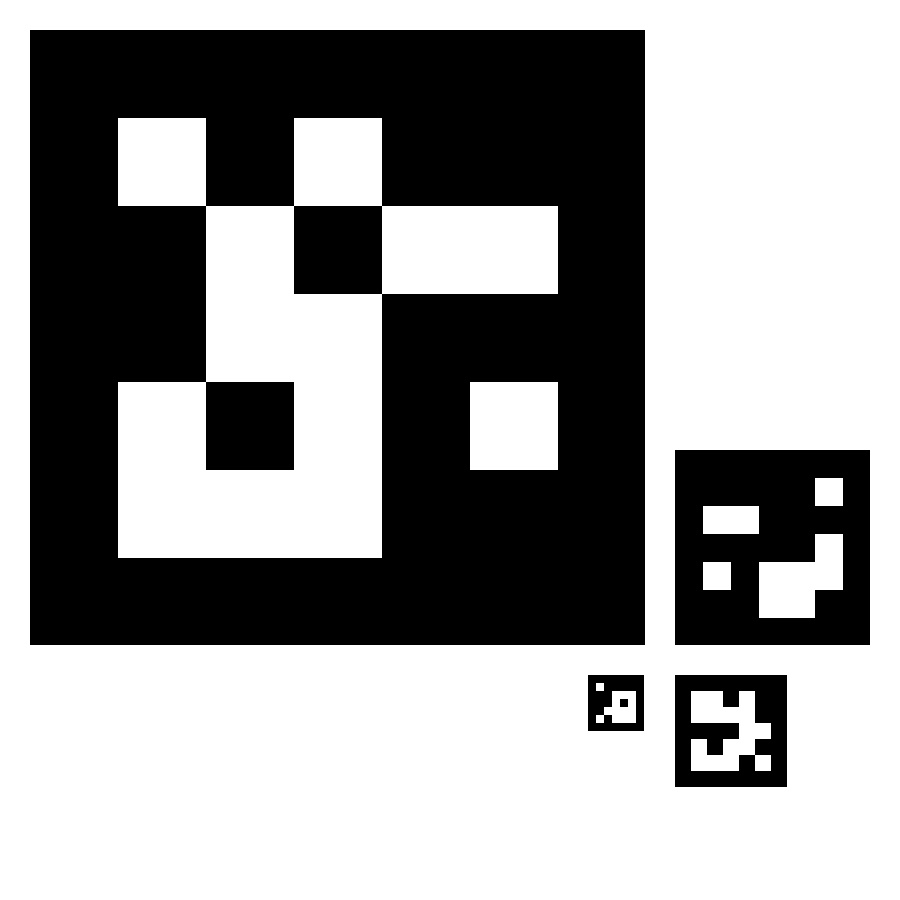
\includegraphics[width=.8\linewidth]{img/ArUco_recursive.jpg}
	  \captionof{figure}{Example of RAM}
	  \label{fig:ArUco_recursive}
	\end{minipage}%
	\begin{minipage}{.5\textwidth}
	  \centering
	  
\includegraphics[width=.8\linewidth]{img/ArUco_pixel_replacement.png}
	  \captionof{figure}{Example of PRiAM}
	  \label{fig:ArUco_pixel_replacement}
	\end{minipage}
\end{figure}

%\subsection{Camera and Optics} % (fold)
%\label{sub:camera_and_optics}
%Selection of camera lens
%camera pixel pr tag pixel at different heights.
%Camera calibratin matrix

% subsection camera_and_optics (end)